\documentclass[conference]{IEEEtran}
\IEEEoverridecommandlockouts
\usepackage{algorithmic}
\usepackage[backend=bibtex,style=ieee,natbib=true]{biblatex}
\usepackage{graphicx}
\usepackage{textcomp}
\usepackage{xcolor}
\usepackage{xurl}

\addbibresource{main.bib}

\begin{document}

\title{
    COMPSCI 402 --- Artificial Intelligence\\
    Final Report\\
    The Development and Outlook of AI Techniques in The Field of
    Practical Federated Learning on Mobile Devices
}

\author{
    \IEEEauthorblockN{Sichang He}\\
    sichang.he@dukekunshan.edu.cn
}

\maketitle

\begin{abstract}
% TODO: Insert a very brief paragraph to summarize your essay
\end{abstract}

\section{Introduction}

% Briefly introduce your understanding of AI,

The term ``artificial intelligence'' (AI) is used to refer to
artificial machineries that
resembles human intelligence in either the way they function or
the way they behave.
These machineries, or intelligent agents,
are not limited to,
but are often designed and built in the form of computer software programs that
run on general purpose computer hardware.

Machine learning (ML), being a significant topic in AI,
refers to the study of intelligent agents that are able to
adapt to previously unseen situations based on data from the past.
The process where an intelligent agent analyzes data from the past to
prepare its abilities is referred to as ``learning'', or ``training''.
Therefore, the data from the past is referred to as ``training data''.
Once the training is complete,
the agent would be able to make predictions or decisions,
or ``make inferences'',
when facing situations that may potentially not be previously seen.
To achieve ML, the common approach is to build a model,
a program that implements some mathematical function,
and train this model by altering the parameters in the function.

% provide an overview of the application of the AI in your research area.
% For example, you can discuss the current development trend and
% provide a roadmap of the development of AI techniques in your research area.

Federated learning (FL), first proposed in 2016, is an ML technique that
allows distributed intelligent agents to collaborately train a model using
their local data~\cite{mcmahan2017communication,yang2019federated}.
These private data are kept local,
therefore FL is suitable for scenarios where
the training data cannot be shared to a central intelligent agent due to
privacy restrictions.

The increasing need to train ML models for business,
the rising awareness of data privacy among individuals,
and the improving laws of governments contribute to
the growing applications of FL.
FL is a compelling option for companies to train ML models using users' data
without breaking some of the privacy laws.

The applications of FL broadly concerns with situations where
the private data that individual intelligent agent possesses are in
the center of the problem.
Some of the earliest practical applications of FL are proposed
in~\cite{bonawitz2019towards},
including selecting and ranking items, suggesting relevant content,
and next-word prediction for smart keyboard on mobile devices.
In all these applications,
the private data from the users' interactions with
the keyboard are in the center of the problems.
Since then, a large portion of practical applications of FL have been
focusing on applications on mobile devices.
For example, vision-based product quality inspection~\cite{bharti2022edge} using
an iOS application and
SMS spam classification on Android devices~\cite{sriraman2022device}.

Despite the advantages of mobile FL on paper,
the practical applications of FL on mobile devices are still limited.
FL is proposed in as early as 2016~\cite{mcmahan2017communication},
and the first effective and well-known application of FL
was announced in 2019~\cite{bonawitz2019towards},
yet, in 2023, FL applications are still rare to see.
The reason is that practical FL faces many challenges such as
privacy security, training efficiency and performance issues,
and heterogeneity problems~\cite{wen2023survey}.

\section{The General Procedure of Federated Learning on Mobile Devices}

% TODO: Expand this.
Generally, FL involves a distributed system that
consists of two parties of intelligent agents and
four phases per training iteration.
The two parties are the central server and the clients.
From the perspective of the ML models being trained,
for each iteration,
the global model is distributed to the clients from the central server;
then, the clients train it locally using local training data;
after local training,
the clients send the trained local models back to the central server;
finally, these local models are aggregated into a new global model,
and the process is potentially repeated for the next new iteration.
For FL on mobile devices,
the clients are typically mobile applications running on Android or iOS devices,
and the central server is a remote server on the Internet,
as illustrated in Fig.~\ref{fig:general-fl}.

\begin{figure}
\centerline{
    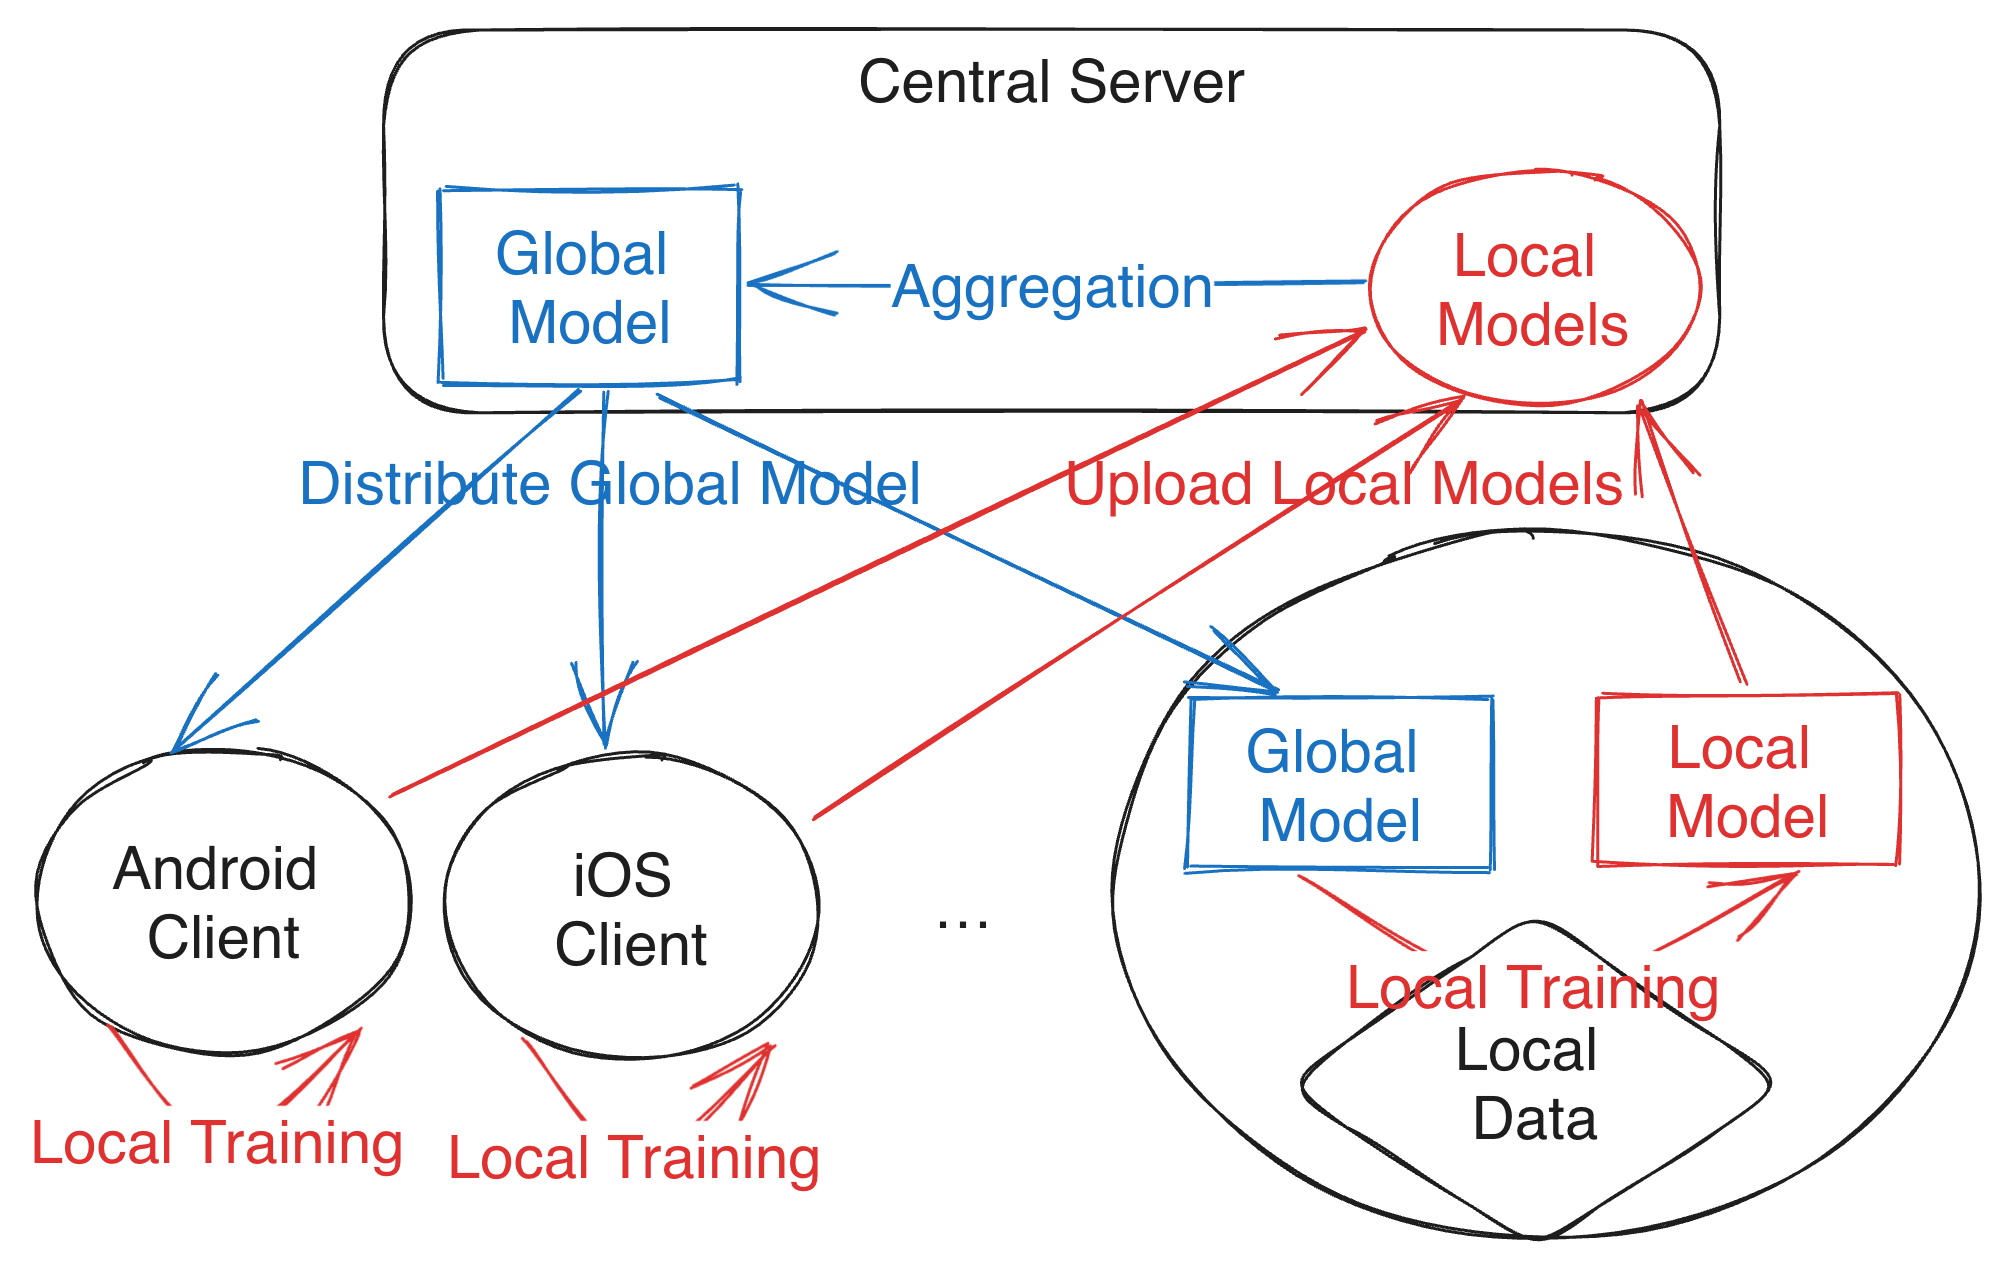
\includegraphics[width=0.5\textwidth]{general-fl.png}
}
\caption{General Procedure of FL for Mobile Devices.}
\label{fig:general-fl}
\end{figure}

The specific implementations of FL on mobile devices vary,
but they all have a similar basis that we discuss in the following.

\subsection{The FedAvg Algorithm}

The first FL algorithm ever, \verb|FedAvg|,
is proposed in~\cite{mcmahan2017communication}.
It is also the most typical FL algorithm,
with many of its aspects regarded as the standard FL procedures.
Many other FL scheduling strategies are only different from \verb|FedAvg| in
minor details.

In \verb|FedAvg|,
we assume $K$ fixed number of clients,
where each client $k$ has a fixed partition $P_k$ of
the total training data ($k \in \{1, 2, \dots, K\}$) as their local data.
For efficiency,
in each iteration $t$ of the training process,
the central server randomly samples $C$ clients for local training.
Each selected client $k$ obtains the parameters $w^{(t)}$ of
the latest global model from the server,
and then train the model locally using their local data $P_k$
produce a new local model.
The objective of this local training process is to minimize the loss $L$ of
the model with parameters $w_k$ for partition $P_k$:
\begin{equation}
    \min_{w_k} L(P_k;w_k).
\end{equation}
The local training is scheduled for a fixed number of $E$ epochs.
And, it produces a new set of weights $w_k^{(t+1)}$ for
each selected client $k$.

To aggregate the local models and derive a global model that
is optimized for all training data $\bigcup_k P_k$,
the objective for the global model is set to
\begin{equation}
    \min_{w} \frac{\sum_k |P_k|L(P_k;w)}{\sum_k |P_k|}
\end{equation}
where $|P_k|$ is the size of partition $P_k$.
To approach this objective,
\verb|FedAvg| aggregates the parameters of local models by
taking the weighted average:
\begin{equation}
    w^{(t+1)}=\sum_k \frac{|P_k|}{\sum_k |P_k|}w_k^{(t+1)}.
\end{equation}

The above iteration step is repeated many times until
the experiment is terminated or
the model has converged.

\verb|FedAvg| has been shown to be effective and practical
in experiments~\cite{mcmahan2017communication}.
Specifically, it was benchmarked against \verb|FedSGD|\cite{chen2016revisiting},
an older algorithm designed for distributed ML,
in a data center setting~\cite{bonawitz2019towards}.

\subsection{The Specific Challenges of Practical Federated Learning on
Mobile Devices Under the FedAvg Context}

However, FL on mobile devices differs significantly from
FL in a data center setting.
Mobile devices are a distinct kind of intelligent agents compared to
servers in data centers.
They are highly heterogeneous,
composing of a wide range of hardware and software configurations.
Thus, problems arise when applying \verb|FedAvg| to FL on mobile devices in
practical scenarios.

FL on mobile devices require customized scheduling.
\verb|FedAvg| waits for each client to finish in each iteration.
Mobile clients differ greatly in their computational abilities,
therefore some of them are bound to be much slower than others.
This often causes the problem where
a small number of clients lag behind all other clients,
known as
``the straggler problem''~\cite{chen2020asynchronous,zheng2017asynchronous}.
The straggler problem significantly decrease the training efficiency of FL,
and are initially mitigated by backup workers~\cite{chen2016revisiting}.
This mitigation strategy, however,
is not suitable for FL on mobile devices because
each client typically possesses a different set of data.
Novel scheduling strategies are developed to
make FL on mobile devices more efficient.

FL on mobile devices faces significant challenges in communication.
\verb|FedAvg| involves transmitting all the model parameters among
clients and the server.
For FL on mobile devices,
clients usually connect to the server via wireless networks,
limiting the transmission bandwidth and reliability.
Various techniques are developed to reduce the amount of data transmitted
and improve the reliability of the transmission.

The final problem that prevents practical FL on mobile devices is
the problem of on-device training.
To start with, the ability to train ML models on mobile devices has been
bleeding-edge and
is on-device training is not generally well-supported on any mobile platform.
Additionally,
while \verb|FedAvg| assumes that all the model parameters are
in the same format that is known to all agents involved,
for FL on mobile devices,
the training on the devices usually involves platform-specific ML frameworks
that differ from the ones on the server.
This parameter alignment problem doubles when
the mobile client run on different platforms with
different ML frameworks.
To solve the on-device training problem,
various ML frameworks are experimented with,
and some FL frameworks developed their own training implementations.

\section{Customizations in Federated Learning Scheduling Strategies for
    Mobile Devices
}

The heterogeneity of mobile devices means that FL on mobile devices needs to
adopt custom scheduling strategies.
If only \verb|FedAvg| is applied,
the most inefficient client would be the bottleneck of
the whole training process.
For example, one person with a five-year-old Android phone may determine
the training efficiency of the whole FL system.

\subsection{Mitigating the Straggler Problem}

The typical settings for the original \verb|FedAvg| can be changed in
various ways for different FL needs.
For example,
the sampling of clients can be changed to a function based on
each client's properties instead of being random,
and the number of clients sampled each iteration could vary.
Also, the aggregation of the local parameters could use another function.

Some strategies to mitigate the straggler problem have been proposed.
A timeout could be applied to drop
straggling devices~\cite{bonawitz2019towards}.
However, this strategy is not suitable for FL on mobile devices because
some devices may be inherently slower than others and
their training data would be wasted.

Most strategies to mitigate the straggler problem involve
synchronous aggregation.
\verb|FedProx|~\cite{li2020federated} is proposed to
allow for each client to train for a various number of local epochs according to
their computational abilities.
\verb|FedProx| has been shown to be much more efficient than
\verb|FedAvg| in heterogeneous settings.
It has been widely supported in FL frameworks designed for simulations and
benchmarks, such as
TensorFlow Federated~\cite{tff},
Syft~\cite{ryffel2018generic,Ziller2021,hall2021syft}, and
LEAF~\cite{caldas2018leaf}.
Other similar optimizations include
\verb|ef-signSGD|~\cite{karimireddy2019error},
\verb|FedAdam|~\cite{reddi2020adaptive},
and~\cite{luo2021cost}.

\newcommand{\FedML}{FedML~\cite{he2020fedml}}
\newcommand{\Florida}{Project Florida~\cite{madrigal2023project}}

On the other hand,
instead of using strict iterations,
the training process could also be
asynchronous~\cite{chilimbi2014project,zhu2022online,huba2022papaya}.
Asynchronous aggregation has been adopted in
FL frameworks like \FedML{} and \Florida{}.

\subsection{Testing FL Scheduling Strategies}

Many FL frameworks are developed for production-level FL simulations to
experiment with scheduling strategies.
TensorFlow Federated~\cite{tff} by Google is widely used as infrastructure for
its rich features.
PaddleFL\footnote{\url{
    https://github.com/PaddlePaddle/PaddleFL
}.} in PaddlePaddle~\cite{ma2019paddlepaddle} by Baidu,
FATE~\cite{liu2021fate} by Tencent, and
OpenFL~\cite{patrick2022openfl} by Intel
are similarly designed for
production-grade FL simulations.
Additionally,
FL benchmarks such as FedScale~\cite{lai2022fedscale} are also developed to
compare and identify scheduling strategies with the highest performance.

\subsection{Implementing Custom Scheduling Strategies}

FL frameworks such as \FedML{} and
Flower~\cite{beutel2020flower} leaves the customization of
scheduling on the client side completely to their users.
From a programming perspective,
these frameworks provide interfaces,
also known as abstract classes,
for custom clients to implement.
These interfaces usually include methods for
training the model locally,
getting and setting the model parameters,
and responding to messages\footnote{\url{
    https://github.com/FedML-AI/FedML/blob/master/android/fedmlsdk/src/main/java/ai/fedml/edge/FedEdgeApi.java
}.}\footnote{\url{
    https://github.com/adap/flower/blob/main/src/kotlin/flwr/src/main/java/dev/flower/android/Client.kt
}.}\footnote{\url{
    https://github.com/adap/flower/blob/main/src/kotlin/flwr/src/main/java/dev/flower/android/Client.kt
}.}.
These interfaces greatly increases the flexibility to
implement custom scheduling strategies when using these FL frameworks,
but they sometimes also leave the burden of implementing them to the users.

While the implementation of the server is usually easily customizable with
open-source frameworks,
the rise of FL as a service (FLaaS)
adds nuances to the server side.
These FLaaS providers manage their own proprietary servers that
are only accessible to the users using opaque APIs or GUIs.
\FedML{}, for example,
offers a set of Python APIs to customize the server implementation,
and allows users to upload their server implementations using a web interface.
\Florida{} is another production-ready FLaaS by Microsoft,
and it supports Python scripts or .NET executables to be uploaded for
server aggregation function.
Both of these FLaaS also provide web GUI interfaces that
are much less customizable.

\section{Communication Implementations Among Clients and the Server}

Remote Procedure Call (RPC) is the standard communication method for
practical FL.
This is likely due to the flexibility it brings to the FL process.
Under an RPC framework,
clients and the server can transfer instructions for the other side to execute.
Therefore, RPC allows for straightforward customization of
FL schedule strategies.

\FedML{} uses an abstract communication layer on top of
the concrete implementations.
These implementations either use the message passing interface
(MPI)\footnote{\url{
    https://www.mpi-forum.org/
}.} over HTTP,
or uses the MQTT protocol\footnote{\url{
    https://mqtt.org/mqtt-specification/
}.}.

The gRPC Remote Procedure Call\footnote{\url{
    https://grpc.io/
}.} is another popular choice for FL communication.
It is used by TensorFlow Federated~\cite{tff} and
OpenFL~\cite{patrick2022openfl} for decentralized simulation.
Flower uses gRPC for the standard implementation of
its communication protocol, the Flower Protocol~\cite{beutel2020flower}.
And, \Florida{} allows users to choose between gRPC and REST.

gRPC accompanied by protocol buffers (ProtoBuf)\footnote{\url{
    https://protobuf.dev/
}.} is desirable for communication between FL mobile participants for
several reasons.
ProtoBuf is a compact binary representation for data structures,
allowing for efficient transmission~\cite{popic2016performance},
therefore it is suitable for mobile devices that
are often under restricted network conditions.
gRPC and ProtoBuf are language-agnostic and
provide a wide range of programming language support,
facilitating its adoption on different platforms~\cite{araujo2020performance}.
It is also based on HTTP/2,
therefore it can usually bypass mobile devices' restricted firewalls and
pass through proxies~\cite{araujo2020performance}.
Being connection-based and bidirectional,
gRPC also allows the server to recognize
which clients have lost their connections and
push instructions to the clients.

Syft uses WebSockets for communication between its network-based workers and
the server~\cite{Ziller2021}.

\section{On-Device Training for Federated Learning on Mobile Devices}

Most FL frameworks cannot support practical FL on mobile devices due to
the lack of on-device training support.
These examples include simulation-oriented frameworks such as
TensorFlow Federated~\cite{tff,kholod2020open} and
LEAF~\cite{caldas2018leaf}.
PaddlePaddle~\cite{ma2019paddlepaddle},
only supports inference on Android.

Flower~\cite{beutel2020flower} leaves the on-device training implementation to
its users,
but provides example Android and iOS implementations\footnote{\url{
    https://github.com/adap/flower/tree/main/examples/android-kotlin
}.}\footnote{\url{
    https://github.com/adap/flower/tree/main/examples/ios
}}.

\subsection{First-Party Mobile Machine Learning Frameworks}

Most FL systems utilize existing mobile ML frameworks to
support on-device training.
Google's TensorFlow Lite~\cite{tensorflow2015-whitepaper,abadi2016tensorflow}
for Android is
a popular choice due to its flexibility and
its maturity for on-device training.
For example, TensorFlow Lite is used by FLaaS frameworks such as~\cite{
    kourtellis2020flaas,katevas2022flaas}
for their Android support.
Flower's Android example also uses
TensorFlow Lite~\cite{beutel2020flower,mathur2021ondevice}.
In contrast, Apples's Core ML~\cite{coreml} is less popular because
it is much less user-friendly.
Core ML is only used by a few FL frameworks such as
Flower~\cite{beutel2020flower} for its iOS example,
and is more commonly used for specific applications
such as this vision-based quality inspector application~\cite{bharti2022edge}.

\subsection{Third-Party Mobile Machine Learning Frameworks}

Third-party solutions for these mobile operating systems are less commonly used.
For example, \FedML{} uses
the MNN ML framework~\cite{jiang2020mnn,lv2022walle} by Alibaba for
its on-device training on Android.
MNN claims to support Android and iOS and promises lightweight binaries.
However, in my attempt to use MNN, I found that its documentation is
severely lacking, outdated, and confusing.
Also, despite the claim that MNN supports iOS,
FedML still has not provided an iOS SDK 15 months after they planned
it\footnote{\url{
    https://github.com/FedML-AI/FedML/tree/9aeb0c097efc9ea7037cfe24499c3d61c81c4dca/ios
}.}.

Notably, Syft~\cite{ryffel2018generic,Ziller2021,hall2021syft} developed
its custom on-device training implementations for
both Android and iOS\footnote{\url{
    https://blog.openmined.org/announcing-new-libraries-for-fl-on-web-and-mobile/
}.}.
However, their focus is on security and privacy,
therefore the implementations greatly sacrifice
performance~\cite{ryffel2018generic}.
Furthermore, these custom implementations can only utilize the CPU,
therefore they are far from being practical for real-world applications of
FL on mobile devices.
Unfortunately, development on
both implementations for Android and iOS,
KotlinSyft\footnote{\url{
    https://github.com/OpenMined/KotlinSyft
}.} and SwiftSyft\footnote{\url{
    https://github.com/OpenMined/SwiftSyft
}.} has been inactive for over two years,
indicating that these projects have been abandoned due to a lack of interest.

There are third-party on-device training solutions that are worth keeping an key on,
but the difficulty to interface hardware on different platforms is
still an major challenge.
ONNX Runtime~\cite{onnxruntime} by Microsoft aims to
unify the ML experience on all platforms by
supporting Open Neural Network Exchange (ONNX),
an open-source format to represent deep learning
models~\cite{ParedesdelRio2020}.
However, its implementations are currently only utilizing CPUs,
leaving out the massive performance improvements by the hardware acceleration
from GPUs and NPUs on the processors of modern mobile devices.
This limitation severely restricts its practical usage.

\subsection{Not-For-Mobile Solutions}

Some systems choose to adopt solutions that are not specifically designed for
mobile ML,
including web-based and UNIX-environment-based solutions.
For example,
TensorFlow.js is capable of running inside a browser on mobile devices or
a webview inside mobile applications~\cite{smilkov2019tensorflow}.
The usage of TensorFlow.js by~\cite{sriraman2022device} resulted in
difficulties in testing,
but~\cite{palanisamy2021spliteasy} shows the advantages of TensorFlow.js on iOS
by integrating it into a React Native application for split learning.
Another example is FedScale~\cite{lai2022fedscale},
which uses Termux, a UNIX console on Android,
to run TensorFlow directly.
FedScale's solution is only suitable for its benchmarking purposes because
it requires the Termux application to run and
cannot be embedded.

\subsection{Model Personalization}

Model personalization is another popular variant of FL.
While FL generally aims to train a global model,
in model personalization,
local models are adjusted using each user's data to
adapt to the each specific user.
Therefore, model personalization excels general FL when
facing high statistical heterogeneity among the users~\cite{kulkarni2020survey}.
Model personalization also reduces some restrictions and difficulties that
general FL faces.
For example,
we usually aim to update most or all layers in general FL,
but it is common to only update the last layer of neural networks in
transfer learning,
a type of model personalization.
By only updating the last layer,
model personalization can remain efficient even when
the neural network used is deep;
in contrast, the computational complexity in back propagation for
deep neural networks makes it unsuitable for general FL on mobile devices.
Therefore, general FL either requires smaller models to be used,
or partial updates,
or other techniques to be applied so it does not train the whole model.

% (You can use table to summarize the features of existing methods;
% or you can conduct the comparative study by
% testing some state-of-the-art methods on your selected dataset.)

\begin{table}[htbp]
\caption{Table Type Styles}
\begin{center}
\begin{tabular}{|c|c|c|c|}
\hline
\textbf{Table}&\multicolumn{3}{|c|}{\textbf{Table Column Head}} \\
\cline{2-4} 
\textbf{Head} & \textbf{\textit{Table column subhead}}& \textbf{\textit{Subhead}}& \textbf{\textit{Subhead}} \\
\hline
copy& More table copy$^{\mathrm{a}}$& &  \\
\hline
\multicolumn{4}{l}{$^{\mathrm{a}}$Sample of a Table footnote.}
\end{tabular}
\label{tab1}
\end{center}
\end{table}

\section{Discussion}

% TODO: Provide an outlook on the development of AI technology in
% your research area based on your knowledge of your research area and
% your understanding of AI.
% You can discuss some open challenges and try to
% provide the corresponding potential solutions or
% discuss the potential research directions.

On-device training remains the most significant obstacle for
practical FL on mobile devices.
Although popular FL frameworks such as
PySyft\footnote{\url{
    https://github.com/OpenMined/PySyft/
}.}~\cite{ryffel2018generic,Ziller2021,hall2021syft}
have democratized FL research by providing tooling and
algorithms~\cite{sriraman2022device},
most of them lack comprehensive support for operations on mobile devices.
Among the necessary operations for FL on mobile devices,
on-device training is the most challenging one because
implementing it requires either depending on
platform-specific ML frameworks that are highly experimental (TensorFlow Lite)
or proprietary (Core ML),
or developing home-grown solutions.
Most FL frameworks choose to use platform-specific ML frameworks,
while custom training implementations such as
the Android and iOS implementations of Syft are limited to CPU.
As a result, it is usually difficult to conduct on-device FL
on mobile devices using existing FL frameworks.

Security remains a critical concern in FL.
Attacks to FL systems to reverse engineer the training data have been
demonstrated to be practical~\cite{sun2019really}.
Mechanism that increase anonymity and
reduce the risk of successful attacks have been proposed and implemented.
For example,
homomorphic encryption (HE)~\cite{wang2020homo},
secure multi-party computing (SMC)~\cite{bonawitz2016practical}, and
differential privacy
(DP)~\cite{dwork2006differential,geyer2017differentially} are
adopted by many production-level FL frameworks and
their effectiveness has been demonstrated.
However, the real-world application on mobile devices still faces a fundamental
issue of trust.
After the mobile applications obtain the training data,
there is no obvious way to verify whether the data are used for FL,
or are in fact sent to a central server.
Companies may well use FL to cover their direct data collection under the hood.

\printbibliography

% TODO: at least 10 references,
% 50\% references should be published within 5 years,
% blogs/website/news reports should be less than 10\%.

\end{document}
